\documentclass[letter, 11pt]{article}
%% ================================
%% Packages =======================
\usepackage[utf8]{inputenc}      %%
\usepackage[T1]{fontenc}         %%
\usepackage{lmodern}             %%
\usepackage[spanish]{babel}      %%
\decimalpoint                    %%
\usepackage{fullpage}            %%
\usepackage{fancyhdr}            %%
\usepackage{graphicx}            %%
\usepackage{amsmath}             %%
\usepackage{color}               %%
\usepackage{mdframed}            %%
\usepackage[colorlinks]{hyperref}%%
%% ================================
%% ================================

%% ================================
%% Page size/borders config =======
\setlength{\oddsidemargin}{0in}  %%
\setlength{\evensidemargin}{0in} %%
\setlength{\marginparwidth}{0in} %%
\setlength{\marginparsep}{0in}   %%
\setlength{\voffset}{-0.5in}     %%
\setlength{\hoffset}{0in}        %%
\setlength{\topmargin}{0in}      %%
\setlength{\headheight}{54pt}    %%
\setlength{\headsep}{1em}        %%
\setlength{\textheight}{8.5in}   %%
\setlength{\footskip}{0.5in}     %%
%% ================================
%% ================================

%% =============================================================
%% Headers setup, environments, colors, etc.
%%
%% Header ------------------------------------------------------
\fancypagestyle{firstpage}
{
  \fancyhf{}
  \lhead{
\includegraphics[height=4.5em]{LogoDFI.jpg}}
  \rhead{FI3104-1 \semestre\\
         Métodos Numéricos para la Ciencia e Ingeniería\\
         Prof.: \profesor}
  \fancyfoot[C]{\thepage}
}

\pagestyle{plain}
\fancyhf{}
\fancyfoot[C]{\thepage}
%% -------------------------------------------------------------
%% Environments -------------------------------------------------
\newmdenv[
  linecolor=gray,
  fontcolor=gray,
  linewidth=0.2em,
  topline=false,
  bottomline=false,
  rightline=false,
  skipabove=\topsep
  skipbelow=\topsep,
]{ayuda}
%% -------------------------------------------------------------
%% Colors ------------------------------------------------------
\definecolor{gray}{rgb}{0.5, 0.5, 0.5}
%% -------------------------------------------------------------
%% Aliases ------------------------------------------------------
\newcommand{\scipy}{\texttt{scipy}}
%% -------------------------------------------------------------
%% =============================================================
%% =============================================================================
%% CONFIGURACION DEL DOCUMENTO =================================================
%% Llenar con la información pertinente al curso y la tarea
%%
\newcommand{\tareanro}{7}
\newcommand{\fechaentrega}{21/11/2020 23:59 hrs}
\newcommand{\semestre}{2020B}
\newcommand{\profesor}{Valentino González}
%% =============================================================================
%% =============================================================================


\begin{document}
\thispagestyle{firstpage}

\begin{center}
  {\uppercase{\LARGE \bf Tarea \tareanro}}\\
  Fecha de entrega: \fechaentrega
\end{center}


%% =============================================================================
%% ENUNCIADO ===================================================================

\noindent{\large \bf Problema 2}

Integre la ecuación de Poisson para el potencial electrostático:

$$\nabla^2 V(x, y) = -\rho(x, y)$$

\noindent donde $\rho(x, y)$ es la densidad de carga.  Integre dentro de una
caja rectangular de dimensiones 10 [cm] $\times$ 15 [cm] conectada a tierra (es
decir, $V = 0$ en el perímetro). Definiremos el centro de la caja como $(x, y)
= (0, 0)$. Dentro de la caja hay una linea que une los puntos $(x_0, y_0) =
(-3, -5.5)$ y $(x_f, y_f) = (3, -5.5)$ que cumple con condiciones de borde
derivativas:

$$ \frac{\partial V}{\partial y} = -1~({\rm sobre~la~línea})$$

\noindent Además, en la caja hay una letra, la primera letra de su nombre.
Dicha letra está contenida dentro del rectángulo centrado con lados 5 [cm]
$\times$ 7 [cm] en las direccione $x$ e $y$, respectivamente.  Dibuje la letra
como quiera, pero intente hacerla lo más simple posible y en particular evite
lineas curvas y diagonales.  El grosor de las líneas que dibujan su letra debe
ser de 1 [cm]. La carga total dentro de la letra es:

$$Q = \int \rho(x, y) dx dy = 2.XXX~[C]$$

\noindent (la unidad es el Coulomb), $XXX$ son los 3 últimos dígitos de su RUT
y la densidad de carga es constante dentro de la letra. A continuación un par
de ejemplos de letras complicadas (sólo como referencia, Ud. puede dibujarlas
como mejor le parezca). La línea roja es donde se aplica la condición de borde
derivativa. El rectangulo verde es el que contiene a la letra. Las líneas
punteadas marcan el centro de la caja.


\begin{center}
  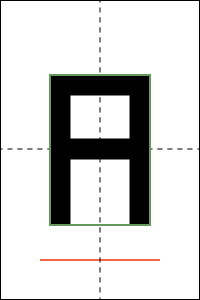
\includegraphics[height=20em]{A.png}
  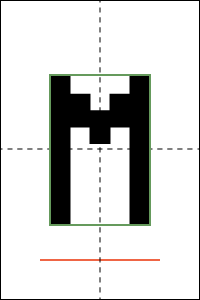
\includegraphics[height=20em]{M.png}
\end{center}


\pagebreak

\begin{itemize}

  \item Use un reticulado con $h\sim0.1~{\rm [cm]}$.

  \item Note que tendrá que derivar el algoritmo de iteración para los puntos
    adyacentes al segmento con condición de borde derivativa y para el
    segmento mismo.  Debido a esto, es recomendable separar la iteración en
    distintos segmentos

  \item Use el método de sobre-relajación sucesiva con distintos $w$ y
    estudie cuantas iteraciones hacen falta para converger en cada caso.

  \item Debe definir un criterio de convergencia, explicítelo en el informe.

  \item Se recomienda que parta con un setup simple y vaya agregando
    complejidad, asegurándose primero de que los casos simples funcionan. Vaya
    dejando el rastro de su trabajo en \texttt{git}.

  \item Asegúrese de incluír gráficos que demuestren de forma efectiva la
    solución obtenida. Éstos pueden incluir gráficos de superficie en 2D y
    3D, líneas de contorno, cortes transversales, etc. Note que el efecto de
    la letra es muy tenue (la carga es baja) por lo que debe probar
    alternativas para la escala del plot.

\end{itemize}

%% FIN ENUNCIADO ===============================================================
%% =============================================================================

\vspace{2em}
\noindent\textbf{Instrucciones Importantes.}
\begin{itemize}

  \item Evaluaremos su uso correcto de \texttt{python}. Si define una función
    relativamente larga o con muchos parámetros, recuerde escribir el
    \emph{docstring} que describa los parámetros que recibe la función, el
    output, y el detalle de qué es lo que hace la función. Recuerde que
    generalmente es mejor usar varias funciones cortas (que hagan una sola cosa
    bien) que una muy larga (que lo haga todo).  Utilice nombres explicativos
    tanto para las funciones como para las variables de su código. El mejor
    nombre es aquel que permite entender qué hace la función sin tener que leer
    su implementación ni su \emph{docstring}.

  \item Su código debe aprobar la guía sintáctica de estilo
    (\href{https://www.python.org/dev/peps/pep-0008/}{\texttt{PEP8}}). En
    \href{http://pep8online.com}{esta página} puede chequear si su código
    aprueba \texttt{PEP8}.

  \item Utilice \texttt{git} durante el desarrollo de la tarea para mantener un
    historial de los cambios realizados. La siguiente
    \href{https://education.github.com/git-cheat-sheet-education.pdf}{cheat
      sheet} le puede ser útil. {\bf Revisaremos el uso apropiado de la
    herramienta y asignaremos una fracción del puntaje a este ítem.} Realice
    cambios pequeños y guarde su progreso (a través de \emph{commits})
    regularmente. No guarde código que no corre o compila (si lo hace por algún
    motivo deje un mensaje claro que lo indique). Escriba mensajes claros que
    permitan hacerse una idea de lo que se agregó y/o cambió de un
    \texttt{commit} al siguiente.

  \item Para hacer un informe completo Ud. debe decidir qué es interesante y
    agregar las figuras correspondientes. No olvide anotar los ejes e incluir
    una \emph{caption} que describa el contenido de cada figura. Tampoco olvide
    las unidades asociadas a las cantidades mostradas en los diferentes
    gráficos.

  \item La tarea se entrega subiendo su trabajo a github. Clone este
    repositorio (el que está en su propia cuenta privada), trabaje en el código
    y en el informe y cuando haya terminado asegúrese de hacer un último
    \texttt{commit} y luego un \texttt{push} para subir todo su trabajo a
    github.

  \item El informe debe ser entregado en formato \texttt{pdf}, este debe ser
    claro sin información de más ni de menos. \textbf{Esto es muy importante,
    no escriba de más, esto no mejorará su nota sino que al contrario}. La
    presente tarea probablemente no requiere informes de más de 3 o 4 páginas
    en total (dependiendo de cuántas figuras incluya; esto no es una regla
    estricta, sólo una referencia útil).  Asegúrese de utilizar figuras
    efectivas y tablas para resumir sus resultados. \textbf{Revise su
    ortografía}.

   \item Repartición de puntaje: 50\% implementación y resolución del problema
     (independiente de la calidad de su código); 35\% calidad del reporte
     entregado: demuestra comprensión del problema y su solución, claridad del
     lenguaje, calidad de las figuras utilizadas; 5\% aprueba o no
     \texttt{PEP8}; 10\% diseño del código: modularidad, uso efectivo de
     nombres de variables y funciones, docstrings, \underline{uso de git}, etc.

\end{itemize}

\end{document}
